\documentclass[11pt,a4paper]{article}
\usepackage[margin=2.3cm]{geometry}
\usepackage[T1]{fontenc}
\usepackage{lmodern,microtype}
\usepackage{graphicx,booktabs,float,caption,amsmath,array,enumitem}
\usepackage[dvipsnames]{xcolor}
\usepackage[numbers,sort&compress]{natbib}
\usepackage[colorlinks=true,linkcolor=blue!50!black,citecolor=blue!50!black,urlcolor=blue!50!black]{hyperref}
\captionsetup{font=small,labelfont=bf}
\setlength{\parskip}{4pt}
\setlist{nosep,leftmargin=1.4em}
\graphicspath{{../results/figures/}}
\newcommand{\code}[1]{\texttt{\small #1}}

\title{\vspace{-1cm}\textbf{Separating Exoplanets from False Positives in the Kepler Objects of Interest}\\[2pt]
\large Leakage-free machine learning, failure analysis and ranking of unresolved candidates}
\author{Joe Khoury \quad Andy Sleiman \quad Anthony Merhy\\[2pt]
CMPS 261 (Machine Learning), Track A -- American University of Beirut\\[2pt]
Code: \url{https://github.com/AndySleiman/kepler-exoplanet-classification}}
\date{November 20, 2026}

\begin{document}
\maketitle

%--------------------------------------------------------------------
\begin{abstract}
NASA's Kepler telescope flagged 9,564 stars whose brightness dips might be caused by a planet (``Kepler Objects of Interest'', KOIs), but many dips are produced by eclipsing binaries, noise or a neighbouring star. We ask whether machine learning can separate confirmed planets from false positives \emph{using only measurements available before expert vetting}, so that it can help rank which detections deserve follow-up. We remove every column created during vetting (dispositions, the Robovetter score and the four false-positive flags), which would otherwise inflate PR-AUC from 0.955 to 0.998, and split the data by star so that no star appears in both training and testing. We compare logistic regression, random forest, XGBoost, a scikit-learn MLP, a PyTorch residual MLP and an XGBoost+ResMLP ensemble, tuned with 5-fold grouped cross-validation, and add five physically motivated features (for example, whether the transit depth is consistent with the planet-to-star radius ratio). On a held-out test set that was evaluated exactly once, the frozen ensemble reaches PR-AUC 0.968 (95\% CI 0.954--0.979), ROC-AUC 0.982, F1 0.926, and finds 86\% of real planets at 95\% precision. XGBoost alone performs equally well on test. Errors concentrate in weak signals (SNR 10--20), Earth-sized planets, and giant or grazing-transit planets that are rare in the training data. Threshold tuning, calibration, re-weighting and a weak-signal specialist did not improve ranking quality, but deferring the 7\% least certain objects to human vetters roughly halves the error rate on the rest (6.7\% to 3.9\%, validation). Finally, we score the 1,977 unresolved CANDIDATE objects and release the ranked list.
\end{abstract}

%--------------------------------------------------------------------
\section{Introduction}
\textbf{Problem.} The Kepler mission \citep{borucki2010} monitored about 150,000 stars for the small, periodic dimming caused by a planet crossing the stellar disc. Each dip is catalogued as a KOI and is eventually dispositioned as a CONFIRMED planet or a FALSE POSITIVE after a long process of automated and human vetting \citep{coughlin2016,thompson2018}. Objects not yet decided stay CANDIDATE. Vetting is slow, so a model that ranks objects by their likelihood of being real planets could help scientists decide where to spend follow-up time. Earlier work has applied deep learning to Kepler light curves \citep{shallue2018} and machine learning to planet validation \citep{armstrong2021}; here we work on the tabular KOI catalogue.

\textbf{The central difficulty is leakage.} Several catalogue columns are \emph{products} of the vetting process (the disposition itself, the Robovetter score, the false-positive flags). A model that sees them looks near-perfect but would be useless on a new detection. A large part of this project is deciding which variables are legitimate and showing what happens if they are not.

\textbf{Approach.} We (i) audit the columns and keep only 12 physical measurements; (ii) split by star to avoid same-star leakage between training and testing; (iii) build a ladder of models from linear to neural and tune each with grouped cross-validation; (iv) engineer five features that encode physical consistency checks; (v) analyse where the model fails, and test three standard fixes; (vi) evaluate the frozen model once on the held-out test set; and (vii) rank the 1,977 CANDIDATE objects.

\textbf{Main findings.}
\begin{itemize}
\item Leaky columns raise XGBoost's validation PR-AUC from 0.955 to 0.998, so honest evaluation requires removing them (Sec.~\ref{sec:leak}).
\item Five engineered consistency features improve every model family on validation (e.g.\ XGBoost 0.955 $\to$ 0.961).
\item The frozen XGBoost+PyTorch ensemble reaches test PR-AUC 0.968 (CI 0.954--0.979); XGBoost alone ties it, so the extra complexity of the ensemble is not clearly justified on test.
\item Errors concentrate in weak signals, small planets and rare planet types; four model-side fixes did not help ranking quality, whereas \emph{selective deferral} to human vetters does (Sec.~\ref{sec:defer}).
\item Complexity is not worth it here: the neural network and the ensemble add at most +0.004 validation PR-AUC (nothing on test) at 5--37$\times$ the cost and with no interpretability (Sec.~\ref{sec:l2}).
\item A model that sees only pre-vetting measurements ranks 562 of the 1,977 candidates above 0.5, giving a prioritised list for follow-up.
\end{itemize}

%--------------------------------------------------------------------
\section{Dataset and Preprocessing}
\subsection{The NASA KOI cumulative table}
We use the Kepler Objects of Interest cumulative table from the NASA Exoplanet Archive \citep{akeson2013} (snapshot downloaded 6 November 2026; 9,564 rows, 49 columns). Dispositions are 4,839 FALSE POSITIVE, 2,748 CONFIRMED and 1,977 CANDIDATE. Each row describes the transit signal (period, duration, depth, impact parameter, signal-to-noise), the derived planet (radius, equilibrium temperature, insolation) and the host star (effective temperature, surface gravity, radius, Kepler magnitude).

\textbf{Labels.} CANDIDATE objects have no ground truth, so we train and evaluate on CONFIRMED (1) vs.\ FALSE POSITIVE (0): 7,587 objects with 36.2\% positives. The 1,977 CANDIDATEs are kept aside and scored at the end (Sec.~\ref{sec:cand}).

\subsection{Leakage audit}\label{sec:leak}
We drop three groups of columns.
\begin{itemize}
\item \textbf{Vetting outputs:} \code{koi\_disposition}, \code{koi\_pdisposition} (the label itself), \code{koi\_score} (the Robovetter's confidence) and the four false-positive flags \code{koi\_fpflag\_nt/ss/co/ec} (not-transit-like, stellar eclipse, centroid offset, ephemeris match). These are set \emph{after} an object has been examined.
\item \textbf{Identifiers and non-physical fields:} \code{kepid}, names, delivery name, transit epoch, sky position.
\item \textbf{Process signals:} the planet number within the system and the number of KOIs per star, and missing-value indicators. They describe \emph{how} an object was processed rather than its physics: 64\% of objects on multi-KOI stars are confirmed versus 18\% on single-KOI stars, because multi-planet systems are validated statistically in bulk. We also do not use the measurement-uncertainty columns.
\end{itemize}
The remaining 12 features are \code{koi\_period}, \code{koi\_duration}, \code{koi\_depth}, \code{koi\_impact}, \code{koi\_model\_snr}, \code{koi\_prad}, \code{koi\_teq}, \code{koi\_insol}, \code{koi\_steff}, \code{koi\_slogg}, \code{koi\_srad}, \code{koi\_kepmag}.

\begin{figure}[H]\centering
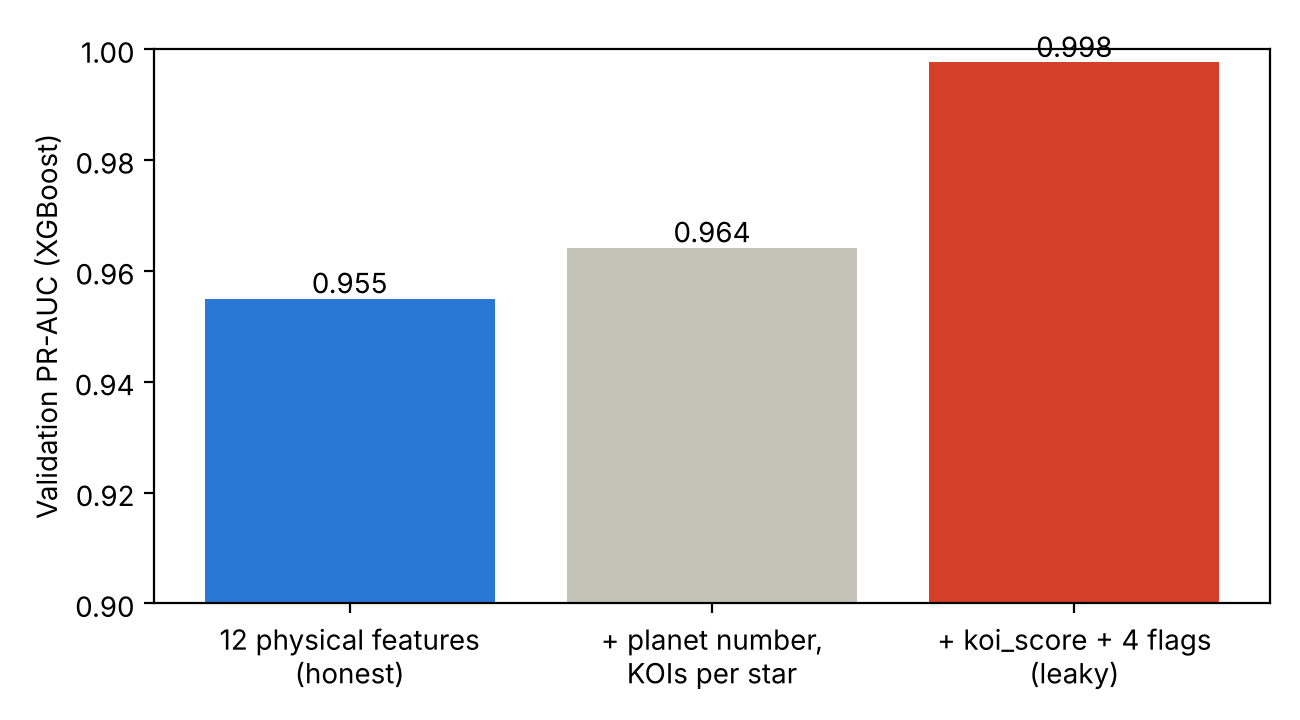
\includegraphics[width=0.62\linewidth]{fig_leakage.png}
\caption{Validation PR-AUC of the same tuned XGBoost with different column sets. Adding the vetting columns gives 0.998; a logistic regression on the four flags \emph{alone} already reaches 0.960 and on \code{koi\_score} alone 0.960. Adding process signals gives a smaller but real boost (0.964).}
\label{fig:leak}
\end{figure}

Figure~\ref{fig:leak} shows why the audit matters: the leaky model looks almost perfect, but a model that only repeats the vetting result tells scientists nothing new.

\subsection{Grouped splits}
Several KOIs can orbit the same star (938 of 8,214 stars have more than one). If one is in training and another in testing, the model has effectively seen the star. All splits are therefore \textbf{grouped by star} (\code{kepid}):
\begin{itemize}
\item a 20\% held-out \textbf{test set} (1,546 objects, 1,329 stars), drawn with \code{GroupShuffleSplit} (seed 42) and not used for any choice until the end; no star appears in both parts (verified);
\item a \textbf{train/validation} part (6,041 objects, 5,312 stars) on which all tuning and model selection uses 5-fold \code{StratifiedGroupKFold}.
\end{itemize}
All reported validation numbers are computed on out-of-fold predictions pooled over the five folds.

\subsection{Preprocessing and missing data}
Period, duration, depth, SNR, radius, insolation, stellar radius and temperature are strongly right-skewed, so we apply $\log_{10}$ (clipped at $10^{-3}$). 3.4\% of objects have at least one missing measurement (depth, impact, SNR, radius, temperature, gravity, stellar radius); these are filled with the training median. Logistic regression and the neural networks additionally standardise inputs. Everything is inside a scikit-learn \code{Pipeline}, so every transformation is fitted on training folds only.

Missing values are informative: only 0.8\% of the objects with a missing value are planets. Median imputation hides the missing flag from the model but does not remove the pattern completely (a tree can still isolate the imputed constant); we return to this in Sec.~\ref{sec:limits}.

\subsection{Engineered features}
Five features are computed from the 12 base columns only, and each encodes a physical consistency check that a human vetter would perform (Table~\ref{tab:feats}).
\begin{table}[H]\centering\small
\begin{tabular}{@{}lp{9.2cm}@{}}\toprule
Feature & Meaning\\\midrule
\code{rp\_over\_rs} & planet-to-star radius ratio $R_p/R_\star$\\
\code{depth\_consistency} & observed depth divided by the depth expected from $(R_p/R_\star)^2$; far from 1 when the ``planet'' radius was derived from a contaminated or eclipsing signal\\
\code{star\_density} & relative stellar density $\propto g/R_\star$\\
\code{duration\_ratio} & observed transit duration divided by the duration expected for a central transit around a star of that density ($T\propto P^{1/3}\rho^{-1/3}$); eclipsing binaries on other stars deviate\\
\code{implied\_noise} & noise level implied by depth, SNR and the expected number of transits (weak-signal indicator)\\\bottomrule
\end{tabular}
\caption{New features (logged where appropriate).}\label{tab:feats}
\end{table}

%--------------------------------------------------------------------
\section{Models}
All models are tuned to maximise PR-AUC (average precision) with the same 5 grouped folds. PR-AUC is the primary metric because classes are imbalanced (36\% positive) and the practical task is \emph{ranking} objects for follow-up; we also report ROC-AUC, F1 at 0.5, recall at 95\% precision, and the Brier score. Hyper-parameters are chosen by random search except for logistic regression (grid).

\begin{description}
\item[Logistic regression] (6 values of $C$, balanced class weights). A linear baseline that is fully interpretable. We expected it to fail: the planet rate is not monotonic in the features (very weak \emph{and} very strong signals are mostly false positives), which no single linear boundary can express.
\item[Random forest] (12 configurations: trees, depth, leaf size, features per split). A strong non-linear bagging baseline needing little tuning, robust to skew and outliers.
\item[XGBoost] \citep{chen2016} (40 configurations). Gradient-boosted trees are usually the best performers on medium-sized tabular data and are explainable with exact TreeSHAP values \citep{lundberg2020}. Selected: 200 trees, depth 6, learning rate 0.05, subsample 0.7, minimum child weight 5, $\lambda = 0.5$.
\item[MLP (scikit-learn)] (20 configurations, early stopping). A neural baseline that can learn smooth joint boundaries such as ``a planet-sized depth on a large star''.
\item[PyTorch residual MLP] (10 configurations, then a 5-seed ensemble). A stronger network than the baseline MLP: residual blocks with LayerNorm and SiLU, dropout, AdamW with weight decay \citep{loshchilov2019}, a one-cycle learning-rate schedule \citep{smith2019} and a fixed epoch budget (so the validation fold is never used for early stopping). Selected: width 64, one block, dropout 0.3, learning rate $10^{-2}$, weight decay $10^{-4}$, 40 epochs; implemented in PyTorch \citep{paszke2019}.
\item[Ensemble] The equal-weight average of the XGBoost and ResMLP probabilities. Trees and networks make partly different mistakes, so averaging can reduce variance.
\item[TabPFN (not evaluated).] We planned to test the pre-trained tabular foundation model TabPFN \citep{hollmann2025}. Its weights are gated and could not be downloaded in our compute environment, so \textbf{no TabPFN results are reported}; the script \code{final/run\_tabpfn\_colab.py} is included to run it with the same folds.
\end{description}
Models are implemented with scikit-learn \citep{pedregosa2011}. All code is in one notebook (\code{notebooks/kepler\_final\_notebook.ipynb}) and in the repository, which also contains the trained models for download. \textbf{Model selection rule (fixed before touching the test set):} the primary model is the one with the highest validation PR-AUC.

%--------------------------------------------------------------------
\section{Results}
\subsection{Model comparison and new features}
Table~\ref{tab:main} gives out-of-fold validation results and the single test evaluation for all models. (A re-run of the progress-report models on the repository's data snapshot gives slightly different numbers from those in the progress report, e.g.\ XGBoost 0.955 instead of 0.957, because the snapshot has two more labelled rows and hence a slightly different split. We report the re-run values throughout.)

\begin{table}[H]\centering\footnotesize\setlength{\tabcolsep}{3.5pt}
\begin{tabular}{@{}lcccccc@{}}\toprule
 & \multicolumn{3}{c}{Validation (5-fold grouped CV)} & \multicolumn{3}{c}{Held-out test (once)}\\\cmidrule(lr){2-4}\cmidrule(lr){5-7}
Model & PR-AUC & R@P95 & Brier & PR-AUC & R@P95 & Brier\\\midrule
Logistic regression & 0.726 & 0.000 & 0.159 & 0.759 & 0.022 & 0.154\\
Random forest & 0.943 & 0.650 & 0.063 & 0.958 & 0.785 & 0.057\\
XGBoost & 0.955 & 0.707 & 0.055 & 0.963 & 0.842 & 0.051\\
MLP (sklearn) & 0.952 & 0.693 & 0.059 & 0.964 & 0.777 & 0.052\\\midrule
Logistic regression + new features & 0.736 & 0.000 & 0.156 & 0.767 & 0.048 & 0.151\\
Random forest + new features & 0.955 & 0.721 & 0.056 & 0.963 & 0.830 & 0.051\\
XGBoost + new features & \textbf{0.961} & 0.775 & 0.052 & \textbf{0.968} & \textbf{0.884} & \textbf{0.045}\\
MLP (sklearn) + new features & 0.954 & 0.721 & 0.056 & 0.955 & 0.785 & 0.055\\
PyTorch ResMLP + new features & 0.959 & 0.736 & 0.052 & 0.963 & 0.796 & 0.051\\
\textbf{Ensemble XGB + ResMLP + new} (primary) & \textbf{0.965} & \textbf{0.796} & \textbf{0.049} & \textbf{0.968} & 0.857 & 0.046\\\bottomrule
\end{tabular}
\caption{Validation and test results (R@P95 = recall at 95\% precision). Fold-to-fold standard deviation of validation PR-AUC is about 0.005 for the non-linear models.}\label{tab:main}
\end{table}

\begin{figure}[H]\centering
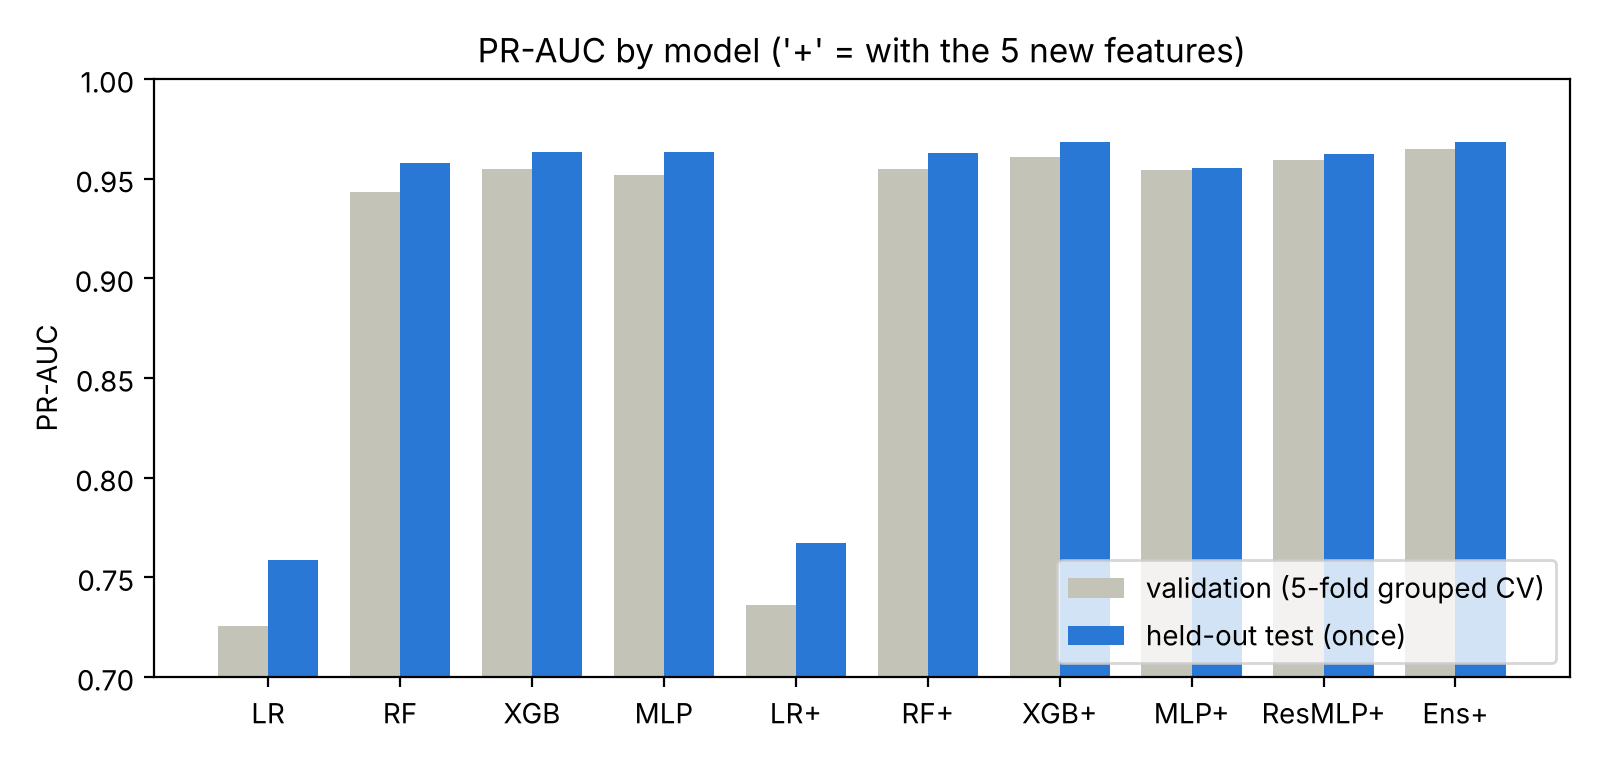
\includegraphics[width=0.85\linewidth]{fig_models_pr_auc.png}
\caption{PR-AUC by model on validation and test.}\label{fig:models}
\end{figure}

Observations.
\begin{itemize}
\item \textbf{Non-linear models are essential:} logistic regression is $\approx 0.2$ PR-AUC behind and cannot reach 95\% precision at all on validation.
\item \textbf{The new features help consistently on validation} (+0.010 logistic regression, +0.012 random forest, +0.006 XGBoost, +0.003 sklearn MLP) and on test for three of four families; the exception is the sklearn MLP, which is lower on test (0.955 vs.\ 0.964), a reminder that single-split differences of $\sim$0.01 are within noise (the test bootstrap interval is $\pm 0.012$).
\item \textbf{The ensemble is best on validation (0.965) but ties XGBoost on test (0.968 for both).} The primary model was frozen on validation, so we report it as primary, but the honest conclusion is that XGBoost with the new features is as good and much simpler.
\end{itemize}

\subsection{Primary model on the held-out test set}
The frozen ensemble (threshold 0.5) reaches PR-AUC 0.968 (95\% CI 0.954--0.979), ROC-AUC 0.982 (0.976--0.987), F1 0.926 (0.909--0.941), recall at 95\% precision 0.857 (0.729--0.917) and Brier 0.046 (0.038--0.054). Intervals come from 1,000 bootstrap resamples of \emph{stars}, so KOIs of the same star stay together. It makes 87 errors on 1,546 objects (45 false alarms, 42 missed planets). Table~\ref{tab:thr} shows the effect of using the two alternative thresholds that were chosen on validation data only.

\begin{table}[H]\centering\small
\begin{tabular}{@{}lcccccccc@{}}\toprule
Threshold & value & precision & recall & F1 & TP & FP & FN & TN\\\midrule
Default & 0.50 & 0.924 & 0.928 & 0.926 & 545 & 45 & 42 & 914\\
F1-optimal on validation & 0.40 & 0.911 & 0.947 & 0.929 & 556 & 54 & 31 & 905\\
95\% precision on validation & 0.80 & 0.956 & 0.809 & 0.876 & 475 & 22 & 112 & 937\\\bottomrule
\end{tabular}
\caption{Test performance of the primary model at three thresholds (chosen on validation).}\label{tab:thr}
\end{table}
The 95\%-precision threshold chosen on validation transfers well: it gives 95.6\% precision on test while keeping 81\% of the planets. The precision--recall curve is in Figure~\ref{fig:prc}.

\begin{figure}[H]\centering
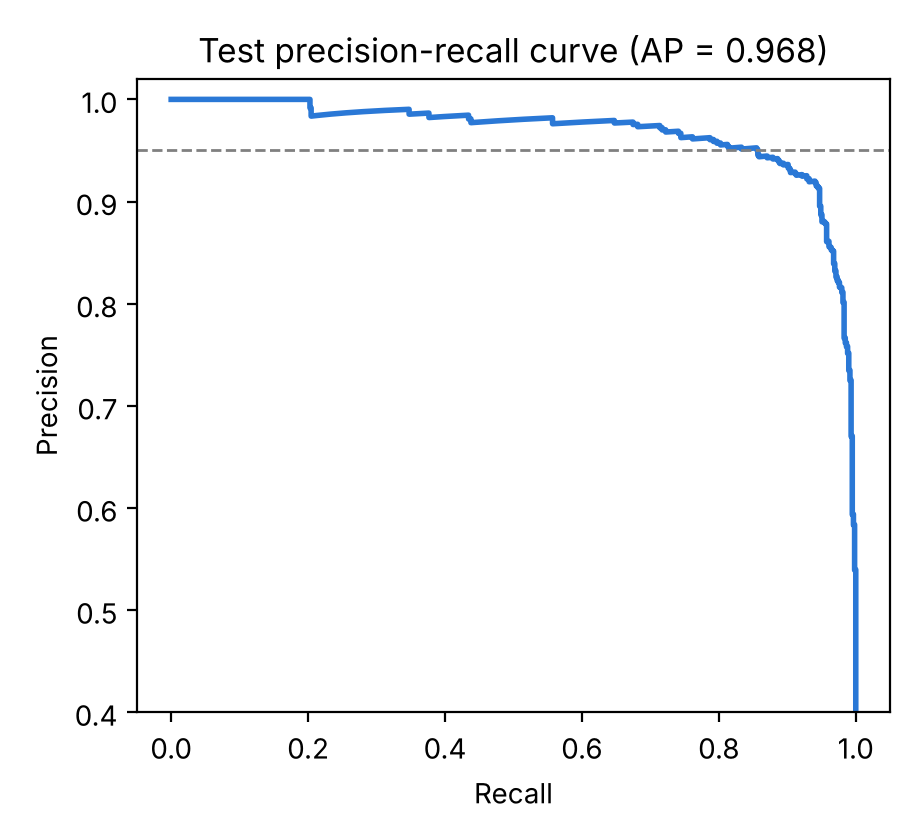
\includegraphics[width=0.45\linewidth]{fig_test_pr_curve.png}
\caption{Precision--recall curve of the primary model on the test set.}\label{fig:prc}
\end{figure}

\subsection{Feature importance (SHAP)}
We computed TreeSHAP values \citep{lundberg2017,lundberg2020} for the XGBoost model (Figure~\ref{fig:shap}). By mean $|$SHAP$|$ (log-odds) the most important features are planet radius (1.14), stellar density (0.82, new), SNR (0.71) and period (0.62), followed by the new \code{depth\_consistency} and \code{duration\_ratio} (both 0.35). Large planet radii, high stellar density and low SNR push predictions strongly towards FALSE POSITIVE. Permuting the 12 raw inputs agrees on the top of the ranking (radius, period, SNR, duration cause the biggest PR-AUC drops; $0.20$, $0.13$, $0.10$, $0.10$). Two of the five new features are among the six most important, which is consistent with their measured gain.

\begin{figure}[H]\centering
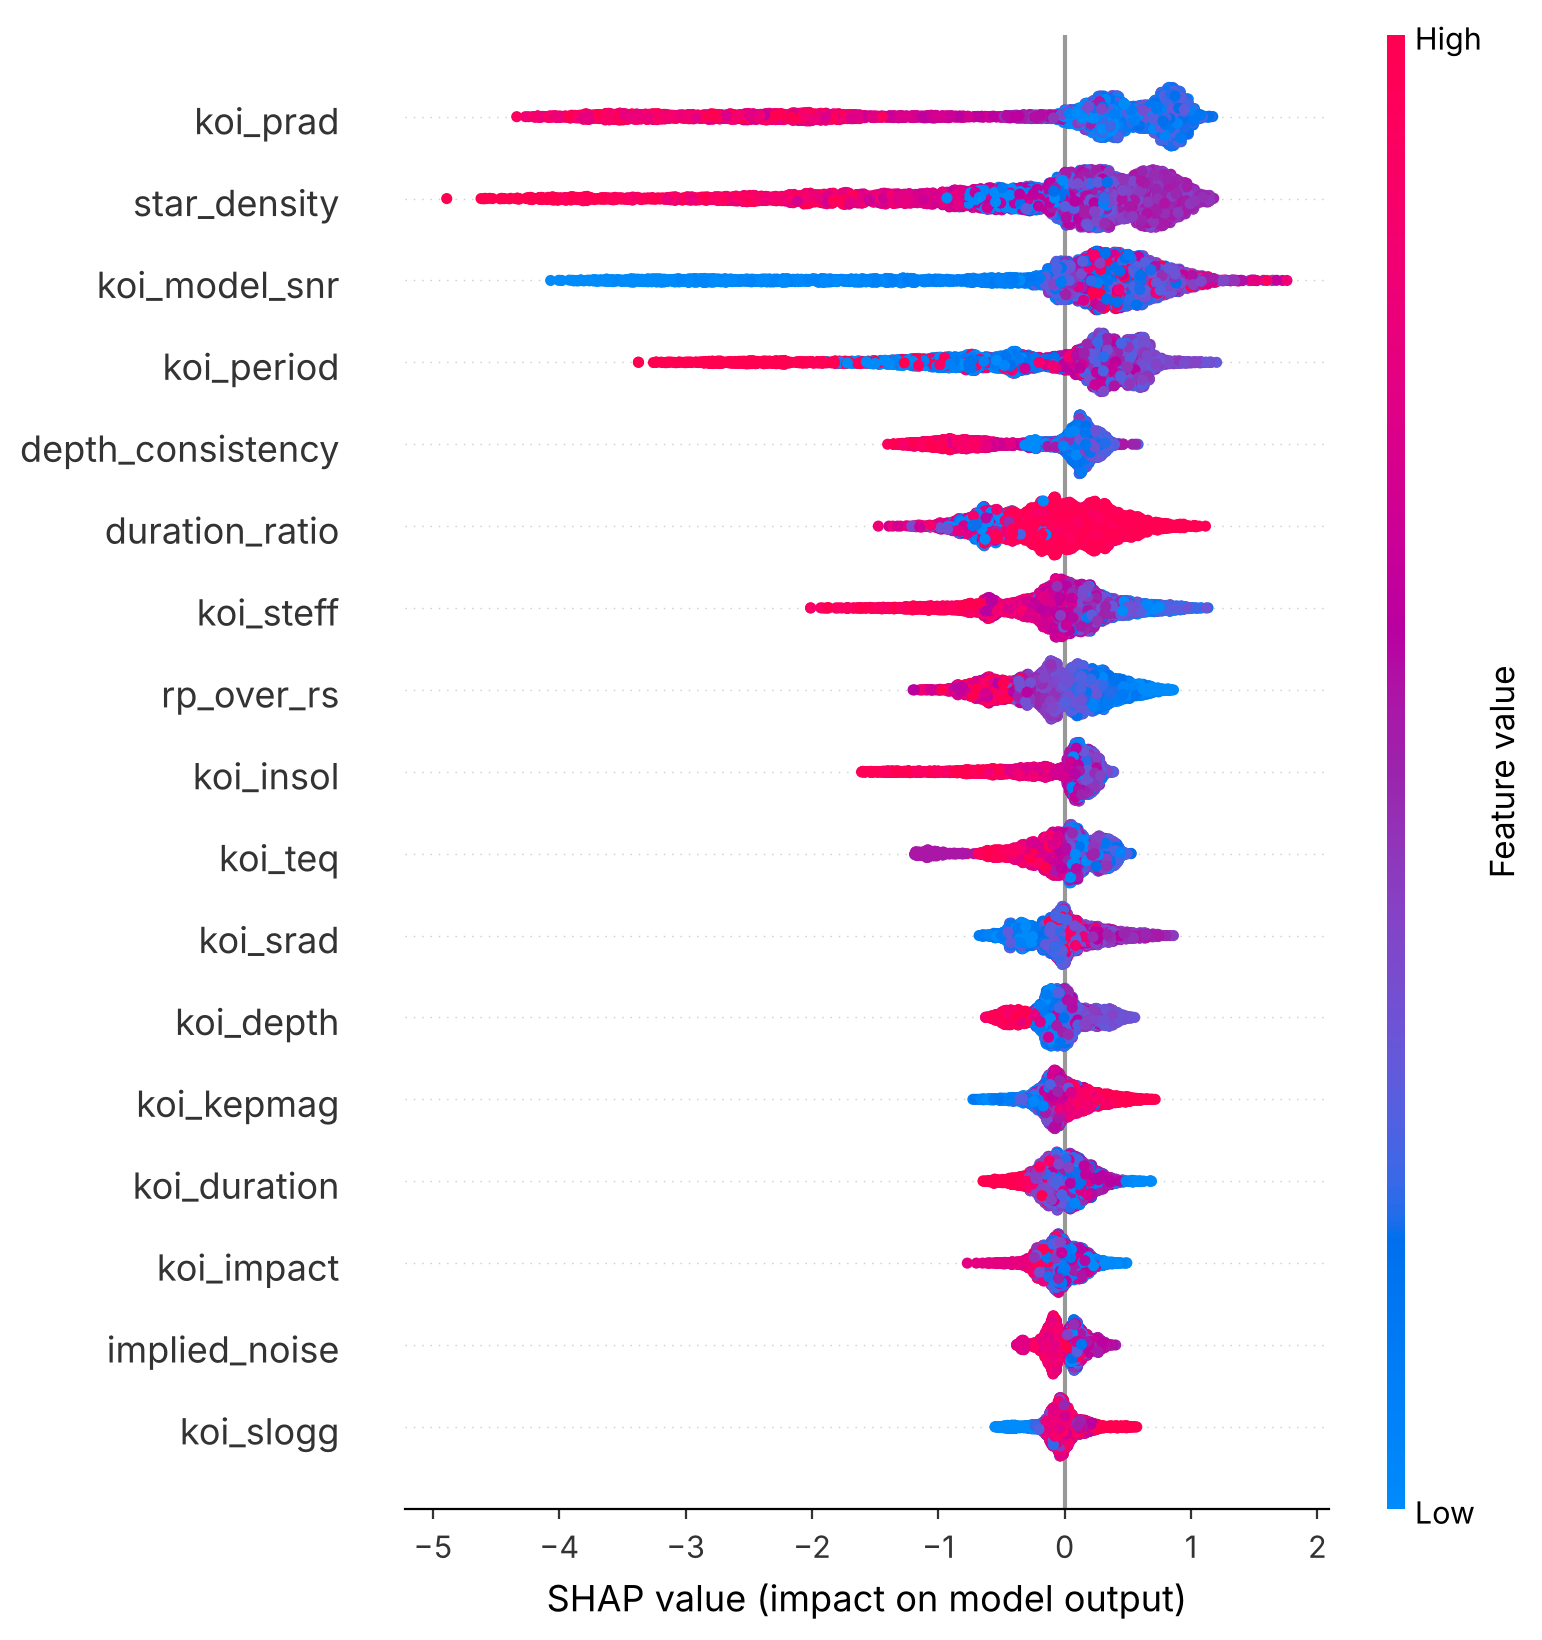
\includegraphics[width=0.48\linewidth]{fig_shap_summary.png}\hfill
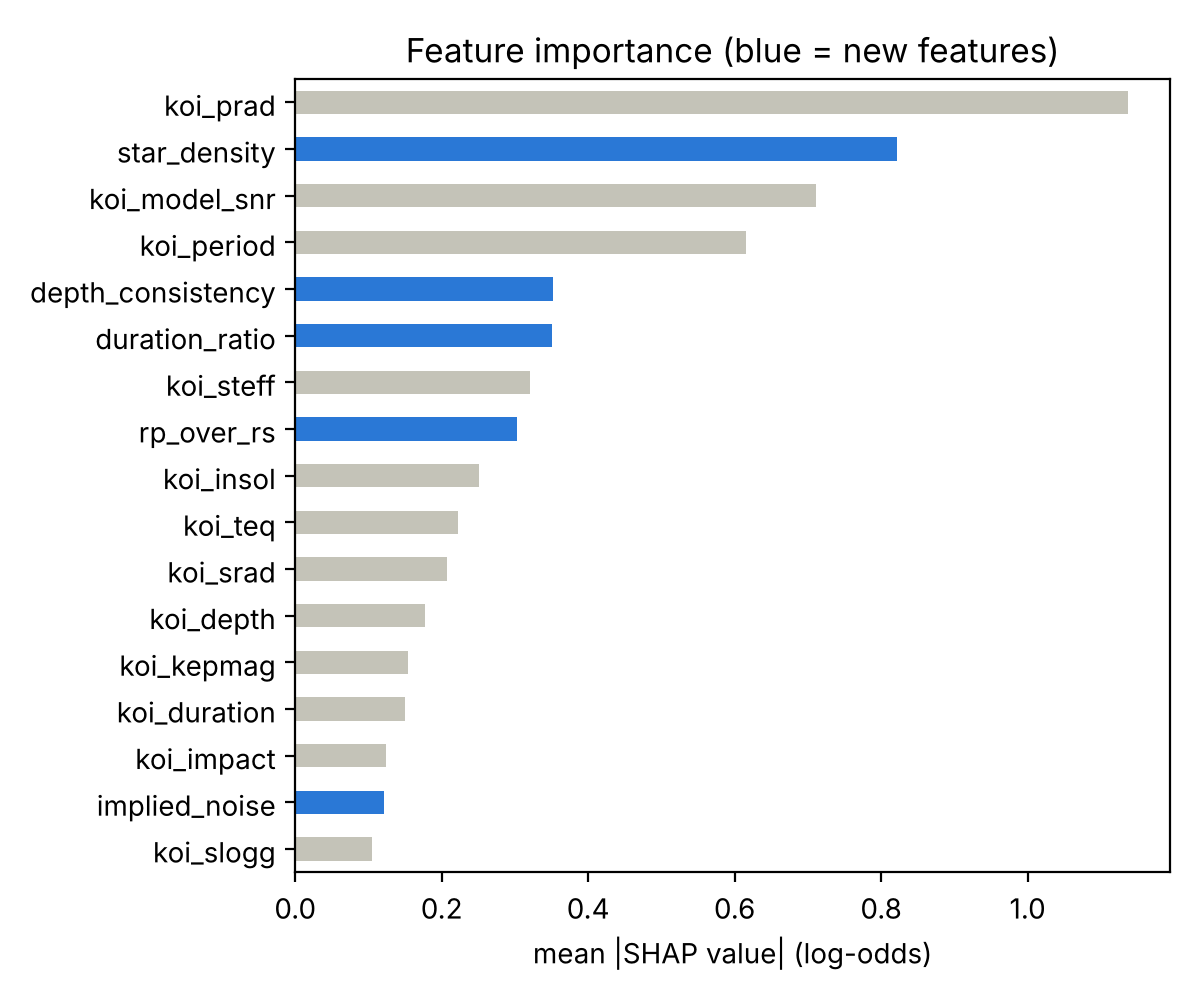
\includegraphics[width=0.48\linewidth]{fig_shap_bar.png}
\caption{Left: SHAP summary of the XGBoost model (each dot is an object; red = high feature value). Right: mean $|$SHAP$|$, new features in blue.}\label{fig:shap}
\end{figure}

\subsection{Complexity analysis}
Table~\ref{tab:cx} compares time, size and interpretability (measured on a 2-core CPU; inference time is per object on a batch of 6,041).

\begin{table}[H]\centering\scriptsize\setlength{\tabcolsep}{2.5pt}
\begin{tabular}{@{}lccccccp{2.9cm}@{}}\toprule
Model & PR-AUC & Size & File (KB) & Tuning (s) & Fit (s) & Infer. ($\mu$s) & Interpretability\\\midrule
Logistic reg. & 0.736 & 18 weights & 3 & 0.9 & 0.08 & 1.8 & High: one coefficient per feature\\
Random forest & 0.955 & 600 trees & 24,413 & 201 & 7.6 & 41.5 & Medium: importances only\\
XGBoost & 0.961 & 200 trees, depth 6 & 399 & 57 & 0.38 & 4.1 & Medium-high: exact TreeSHAP\\
MLP (sklearn) & 0.954 & 1,217 weights & 40 & 97 & 0.81 & 1.9 & Low: black box\\
PyTorch ResMLP & 0.959 & 48,965 weights (5 nets) & 220 & 291 & 13.8 & 2.9 & Low: black box\\
Ensemble & 0.965 & both models & 619 & 347 & 14.2 & 7.0 & Low: black box\\\bottomrule
\end{tabular}
\caption{Validation PR-AUC and cost of each model (all with the new features).}\label{tab:cx}
\end{table}
All models are cheap in absolute terms: scoring the 9,564 objects takes well under a second for every model. The meaningful trade-offs are therefore not speed but \emph{size and interpretability}. The random forest is $60\times$ larger on disk than XGBoost for lower accuracy; the ensemble costs $\approx$ 6$\times$ the tuning time of XGBoost, doubles the model count, is a black box, and bought only +0.004 PR-AUC on validation and nothing on test. XGBoost offers the best balance: near-top accuracy, a 399 KB file, microsecond inference and exact per-object explanations.

\subsection{What does the more sophisticated method improve, and what does it cost?}\label{sec:l2}
\textbf{Improvement.} Against the tuned classical baseline (XGBoost + new features, validation PR-AUC 0.961, test 0.968), the PyTorch ResMLP does \emph{not} improve (0.959 validation, 0.963 test). Averaging the two gives +0.004 validation PR-AUC (0.965) and +0.021 recall at 95\% precision (0.796 vs.\ 0.775), which suggests the networks make partly different mistakes, but on the test set the ensemble's PR-AUC is identical to XGBoost's (0.968) and its recall at 95\% precision is lower (0.857 vs.\ 0.884). The gain is therefore smaller than the fold-to-fold noise (SD $\approx$ 0.005) and the test-set interval ($\pm$0.012).

\textbf{Cost.} Relative to XGBoost, the ResMLP needs 5$\times$ the tuning time (291 s vs.\ 57 s) and 36$\times$ the fit time (13.8 s vs.\ 0.38 s); the ensemble needs 6$\times$ the tuning time and 37$\times$ the fit time, two model files instead of one, and loses exact per-object explanations. Inference speed is not a differentiator (3--7 $\mu$s per object). \textbf{Conclusion:} for this tabular problem the extra complexity is not justified; the classical gradient-boosted model delivers the same test accuracy with a 399 KB file and exact TreeSHAP explanations. We still report the ensemble as primary only because the selection rule was fixed on validation before the test set was opened.

\subsection{Interpretability versus accuracy}\label{sec:interp}
To measure what readability costs, we fitted small decision trees and XGBoost on only the top SHAP features (validation, same folds; Table~\ref{tab:interp}).
\begin{table}[H]\centering\small
\begin{tabular}{@{}lccc@{}}\toprule
Model & Readable size & PR-AUC & Recall@P95\\\midrule
Decision tree, depth 3 & 8 leaves & 0.703 & 0.000\\
Decision tree, depth 4 & 16 leaves & 0.768 & 0.000\\
Decision tree, depth 8 & 256 leaves & 0.891 & 0.000\\
XGBoost, top 3 SHAP features & 3 features & 0.874 & 0.148\\
XGBoost, top 5 SHAP features & 5 features & 0.940 & 0.552\\
XGBoost, top 8 SHAP features & 8 features & 0.955 & 0.723\\
XGBoost, all 17 features & 200 trees & 0.961 & 0.775\\
Ensemble XGB + ResMLP & black box & 0.965 & 0.796\\\bottomrule
\end{tabular}
\caption{Cost of interpretability: a human-readable rule set is far worse than the boosted models.}\label{tab:interp}
\end{table}
A rule set small enough to read (a depth-3 tree) reaches only PR-AUC 0.70, and even 256 leaves reach 0.89, so no \emph{simple} model is competitive: the signal lives in interactions between radius, SNR, period and stellar density. The useful form of interpretability is post-hoc explanation of a boosted model: eight features (about half of the inputs) already retain 99\% of the full XGBoost PR-AUC (0.955 vs.\ 0.961), which is a cheap way to simplify a deployed system.

\subsection{Failure analysis}\label{sec:fail}
We analyse out-of-fold validation predictions of the primary model at threshold 0.5: 403 errors on 6,041 objects (6.7\%), of which 218 are false alarms and 185 missed planets.

\begin{figure}[H]\centering
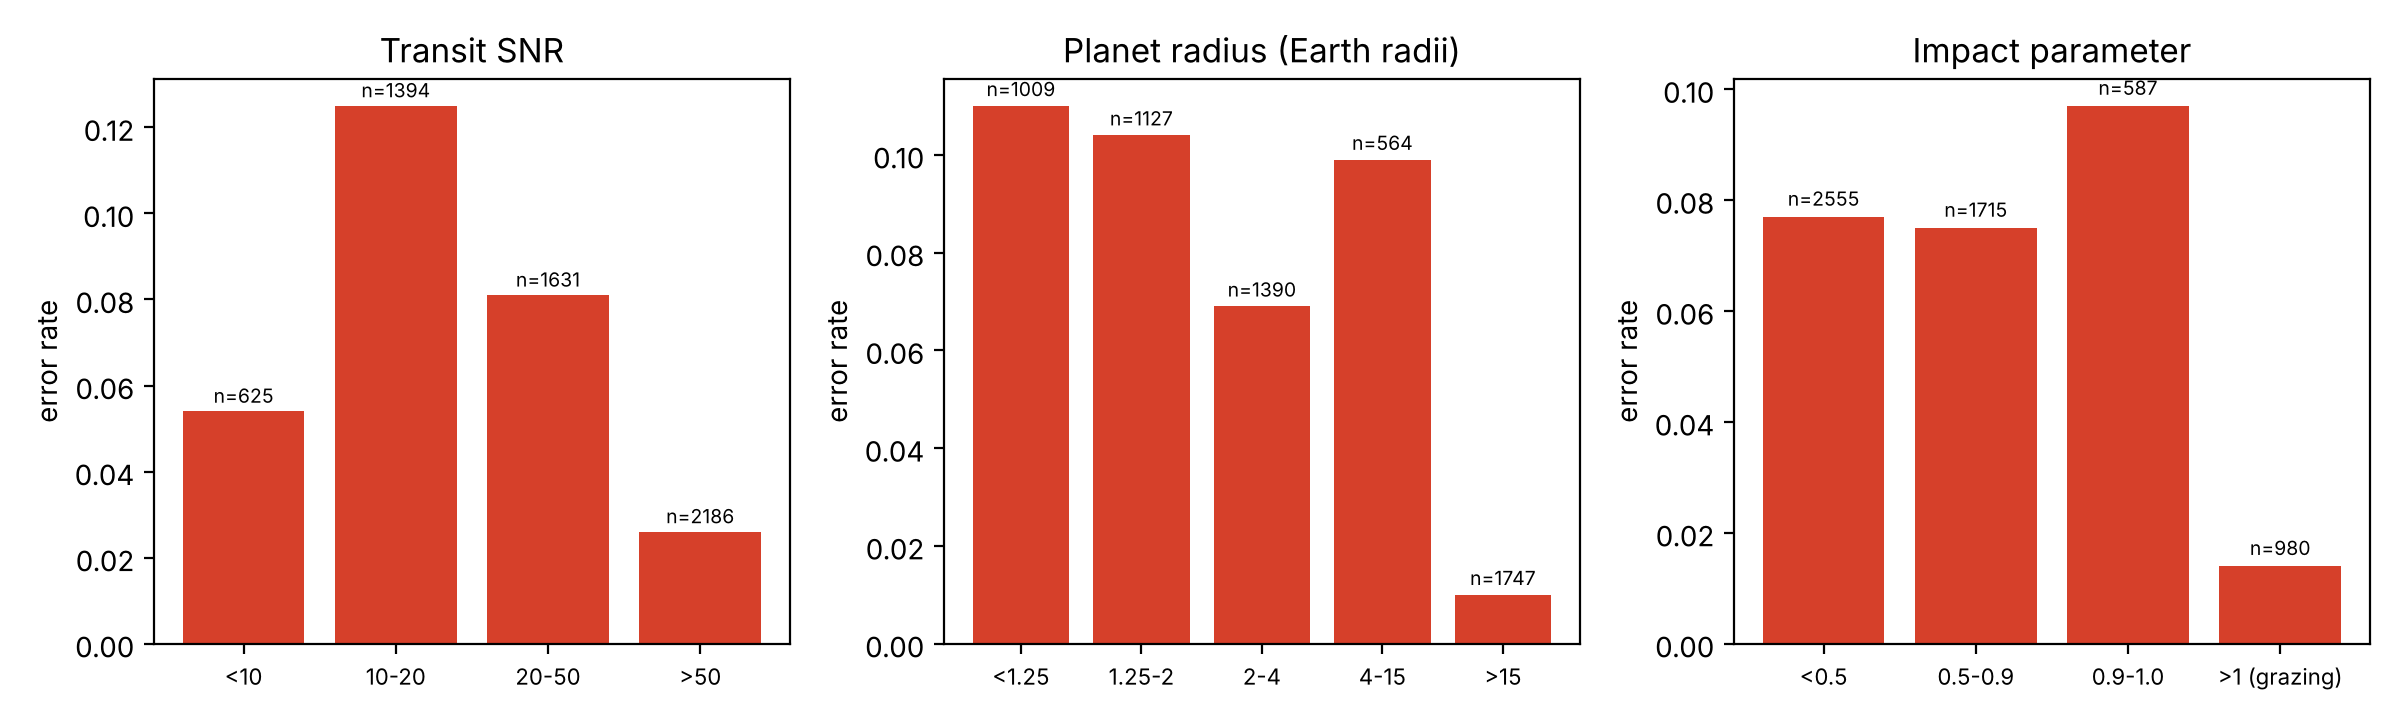
\includegraphics[width=\linewidth]{fig_failure_subgroups.png}
\caption{Error rate of the primary model by subgroup (validation).}\label{fig:fail}
\end{figure}

\textbf{Weak signals.} Errors peak at SNR 10--20 (12.5\% error, 174 of 403 errors, planet rate 40\%): the dip is barely above the noise, so real and fake signals overlap. Below SNR 10 the error rate is low (5.4\%) only because 95\% of these are false positives; ranking within the group is poor (PR-AUC 0.42, 28 of 34 planets missed).

\textbf{Small planets.} Objects below 2 Earth radii have 10--11\% errors (versus 7\% for 2--4 Earth radii) because small real planets look like noise-driven false positives.

\textbf{Rare planet types.} Planets of more than 15 Earth radii are 1.1\% of that group (PR-AUC 0.29, 17 missed planets); grazing transits (impact $>1$) are 1.3\% planets (PR-AUC 0.13); and stars hotter than 6,800 K are 2.6\% planets (PR-AUC 0.45). The error rate in these groups is low, but it is low because the model predicts ``false positive'' almost always, so genuine hot Jupiters and grazing planets are systematically missed. The most confident mistakes are of this type: for example K01450.01 (radius 59 $R_\oplus$, SNR 335, impact 1.23, confirmed) receives probability $0.0003$, and K00013.01 (SNR $\sim$4,000) 0.008.

\textbf{Missing measurements.} The 205 objects with a missing value are 1\% planets (PR-AUC 0.08) and the model labels nearly all of them as false positives. This is correct statistically but reflects the catalogue's processing rather than physics. On the test set, all 55 such objects are false positives and none is misclassified.

\textbf{False alarms that look like planets.} The median false alarm has radius 1.7 $R_\oplus$, SNR 20 and period 8.5 d, close to the median missed planet (1.7 $R_\oplus$, SNR 17, 5.9 d) and unlike rejected false positives (15 $R_\oplus$, SNR 37). The most confident false alarm, K02050.01 ($p = 0.99$; 1.6 $R_\oplus$, SNR 30, period 75 d), is pushed towards ``planet'' by SHAP through its radius, SNR, radius ratio and stellar density, i.e.\ by exactly the features that describe a convincing small transit. Eclipsing-binary and background-star signals that mimic a planet cannot be distinguished using only catalogue measurements; vetting uses extra information such as centroid motion and odd/even depth differences that is not in this table. Short periods ($<3$ d) are also harder (PR-AUC 0.84).

\textbf{On the test set} the same pattern appears: SNR 10--20 has the highest error rate (10.1\%), followed by small planets (8.5--9.2\%), while errors for SNR $>50$ are only 2.1\%.

\subsection{Attempted fixes}\label{sec:fixes}
We tested three standard fixes on validation data. Post-hoc corrections (threshold, calibration) were cross-fitted on out-of-fold predictions to avoid leakage; re-weighting retrains XGBoost with the same hyper-parameters.

\begin{table}[H]\centering\footnotesize
\begin{tabular}{@{}lcccccc@{}}\toprule
Fix (validation) & PR-AUC & R@P95 & Brier & ECE & F1 & errors\\\midrule
Baseline (threshold 0.5) & 0.965 & 0.796 & 0.0488 & 0.0036 & 0.908 & 403\\
Threshold tuned for F1 (0.40) & 0.965 & 0.796 & 0.0488 & 0.0036 & 0.911 & 396\\
Platt calibration & 0.965 & 0.795 & 0.0489 & 0.0036 & 0.907 & 405\\
Isotonic calibration & 0.962 & 0.780 & 0.0493 & 0.0029 & 0.911 & 395\\
Re-weight weak signals (SNR $<20$) $\times 3$ & 0.959 & 0.768 & 0.0524 & 0.0084 & 0.904 & 419\\
Re-weight weak signals and giants $\times 3$ & 0.960 & 0.770 & 0.0522 & 0.0060 & 0.903 & 423\\
Re-weight by inverse class frequency & 0.960 & 0.762 & 0.0519 & 0.0170 & 0.906 & 420\\\bottomrule
\end{tabular}
\caption{Effect of failure fixes on validation data (ECE = expected calibration error).}\label{tab:fix}
\end{table}

\begin{itemize}
\item \textbf{Calibration (can the confidence be trusted?):} yes. The ensemble's reliability curve lies on the diagonal (Figure~\ref{fig:calib}; ECE 0.0036, Brier 0.049), so Platt scaling changes nothing and isotonic regression lowers ECE slightly (0.0029) at a small cost in PR-AUC.
\item \textbf{Thresholds:} the F1-optimal threshold (0.40) removes 7 of 403 validation errors and gives +0.003 F1; on test it gives F1 0.929 vs.\ 0.926. These are within noise. The precision-target threshold is useful operationally (Table~\ref{tab:thr}) because it makes the false-alarm budget explicit.
\item \textbf{Re-weighting} lowers PR-AUC and recall at 95\% precision in every variant and does \emph{not} reduce errors in the SNR 10--20 group (12.5\% $\to$ 12.4--12.6\%). Its only visible ``gain'' (errors in the missing-value group 2.9\% $\to$ 1.0\%) is a trivial effect of predicting ``false positive'' for nearly all of those objects.
\end{itemize}
\begin{figure}[H]\centering
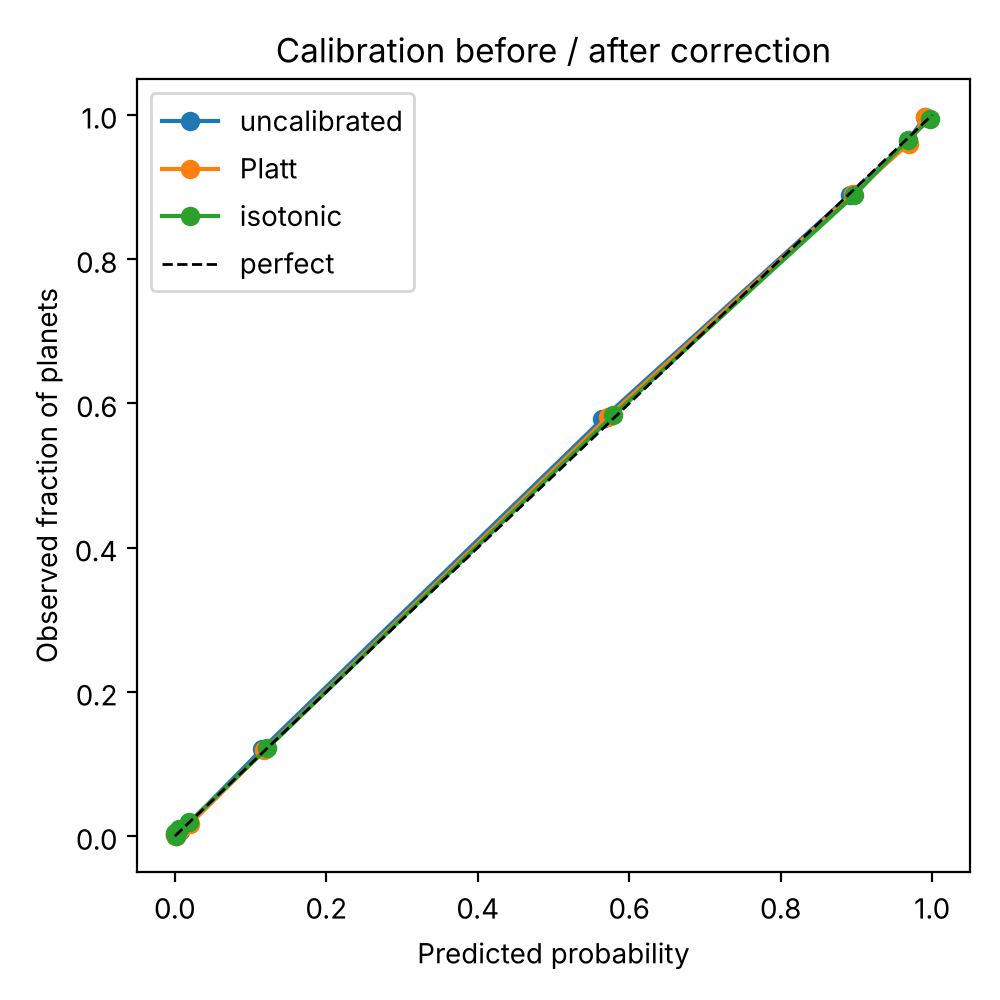
\includegraphics[width=0.42\linewidth]{fig_calibration_fix.png}
\caption{Reliability curve of the primary model (validation, out-of-fold), before and after Platt/isotonic correction.}\label{fig:calib}
\end{figure}
We therefore adopt \emph{none} of these model-side fixes for the primary model (a mitigation that does work is deferral, Sec.~\ref{sec:defer}). The errors are due to genuinely ambiguous signals, not a miscalibrated or biased training objective; improving them needs new information (such as light-curve or centroid features), not re-weighting.

\subsection{Mitigations that work: deferring uncertain objects}\label{sec:defer}
Because the remaining errors come from ambiguous signals, a practical mitigation is \emph{selective prediction}: the model decides only when it is confident and sends objects with probability within a band around 0.5 to human vetters. We also tried a \emph{weak-signal specialist} (an XGBoost trained only on SNR $<30$, averaged with the global model). Both were evaluated on validation out-of-fold predictions only; the test set was not used again.

\begin{table}[H]\centering\footnotesize\setlength{\tabcolsep}{3pt}
\begin{tabular}{@{}lccccc@{}}\toprule
Defer if $|p-0.5|<$ & objects deferred & coverage & error on decided & SNR 10--20 error & errors avoided\\\midrule
0 (no deferral) & 0 & 100\% & 6.7\% & 12.4\% & 0\\
0.05 & 110 & 98.2\% & 5.9\% & 11.2\% & 55\\
0.10 & 219 & 96.4\% & 5.0\% & 9.7\% & 111\\
0.20 & 432 & 92.8\% & 3.9\% & 7.6\% & 184\\
0.30 & 701 & 88.4\% & 3.0\% & 5.5\% & 242\\\bottomrule
\end{tabular}
\caption{Selective prediction (validation). Deferral turns the model into a triage tool: the machine decides the clear cases and humans review the rest.}\label{tab:defer}
\end{table}
Deferring the 7\% least certain objects (band 0.20) removes 184 of 403 errors, halves the error rate on the decided objects (6.7\% $\to$ 3.9\%) and cuts the error rate in the hardest group (SNR 10--20) from 12.4\% to 7.6\%, while still deciding 87\% of the weak-signal objects automatically. The weak-signal specialist, in contrast, changes almost nothing (395 vs.\ 403 errors, SNR 10--20 error 12.0\% vs.\ 12.4\%) and slightly lowers PR-AUC (0.964 vs.\ 0.965), so we do not adopt it. The remaining systematic failures (rare giants, grazing transits and planet-mimicking false positives) need new information rather than a different training objective. These deferral results are validation-only evidence; the band should be re-checked on fresh data before deployment.

\subsection{Ranking the unresolved CANDIDATE objects}\label{sec:cand}
After the test evaluation we refit XGBoost and the ResMLP on all 7,587 labelled objects (frozen hyper-parameters) and scored the 1,977 CANDIDATE objects; the full ranked list is released as \code{results/candidate\_ranking.csv}.

\begin{figure}[H]\centering
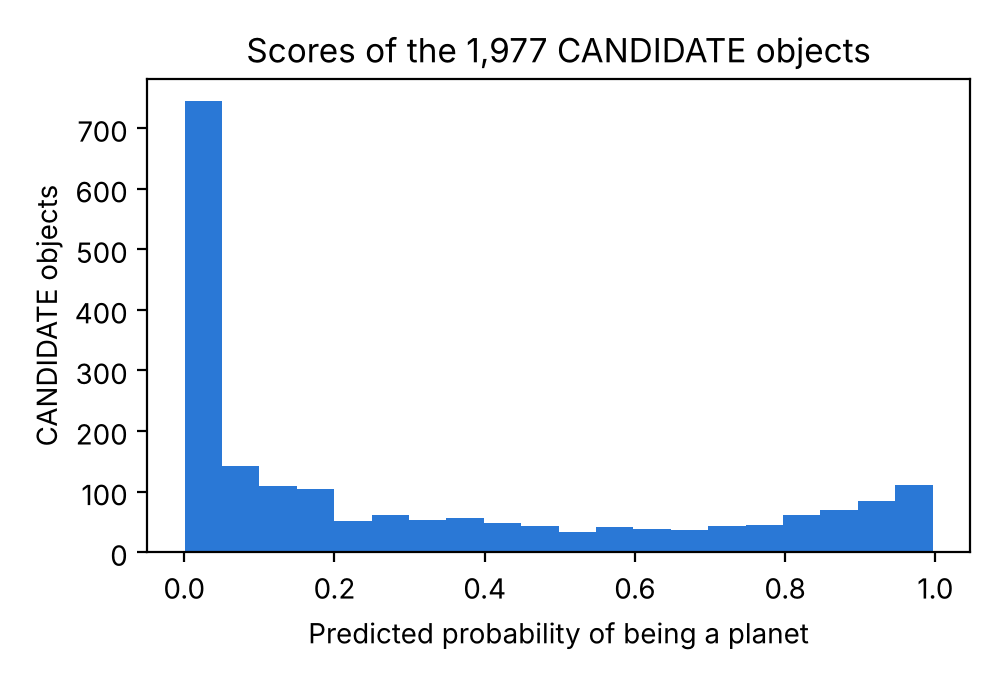
\includegraphics[width=0.5\linewidth]{fig_candidates.png}
\caption{Distribution of planet probabilities for the CANDIDATE objects.}\label{fig:cand}
\end{figure}
The distribution is bimodal: 886 candidates score below 0.1, 562 score at least 0.5 and 325 reach the 0.80 threshold that gave 95\% precision on validation. The top-ranked objects are K01856.01, K00865.01, K01145.01, K01861.01 and K04526.01 (all above 0.99). The ranking agrees only moderately with the NASA Robovetter score (Spearman 0.34, computed after the fact; the score was never used as an input). Candidates are by definition the ambiguous objects, and no ground truth exists, so these scores are a \emph{prioritisation aid for follow-up}, not a statement that these objects are planets.

%--------------------------------------------------------------------
\section{Conclusion}
\textbf{Main results.} Using only 12 pre-vetting measurements and five physically motivated consistency features, a grouped, leakage-free evaluation reaches PR-AUC 0.968 on a held-out test set (ensemble and XGBoost alike), with 86\% of planets recovered at 95\% precision using the ensemble and 88\% using XGBoost. The leakage audit is not a technicality: keeping the vetting columns would report 0.998 for a model that mostly repeats the vetting outcome. Non-linear models are essential, engineered consistency features help every family, and XGBoost offers the best trade-off between accuracy, size and interpretability. Errors concentrate where the data themselves are ambiguous: weak signals, Earth-sized planets, and rare giant or grazing planets, as well as false positives that mimic planets. Model-side fixes did not help, but deferring the 7\% least certain objects to human vetters halves the error rate on the rest, and the extra complexity of neural networks and ensembling is not justified on this tabular data.

\textbf{Limitations}\label{sec:limits}
\begin{itemize}
\item A single grouped split with 1,546 test objects gives wide intervals (e.g.\ recall at 95\% precision: 0.73--0.92), so differences of about 0.01 PR-AUC between models are not significant. The ensemble's validation advantage did not reproduce on test.
\item Median imputation does not fully hide the strong association between missing values and false-positive status, which is a processing artefact; 3.4\% of objects are affected.
\item The ``labels'' (CONFIRMED vs.\ FALSE POSITIVE) come from a vetting process with its own biases, and dispositions in the archive change over time.
\item The TabPFN experiment could not be run (gated weights), and the PyTorch search used only 10 configurations. Deferral and the specialist model were evaluated on validation data only. Interpretability is measured through surrogate/compact models, not with a user study; timings are from a 2-core CPU.
\item Candidate scores have no ground truth and should not be read as confirmations.
\end{itemize}

\textbf{Future work.} (i) Add information that human vetters use but the catalogue lacks: light-curve shape, odd/even depth differences and centroid shifts; (ii) test TabPFN and gradient-boosting variants under the same protocol; (iii) use repeated grouped splits for tighter confidence intervals; (iv) treat the problem as a ranking task with an explicit follow-up budget; (v) examine the confident mistakes (hot Jupiters and grazing planets) with domain experts, and consider a dedicated model for rare planet classes; (vi) track how the candidate ranking compares with future dispositions as the archive is updated.

%--------------------------------------------------------------------
\begin{thebibliography}{99}\small
\bibitem[Akeson et al.(2013)]{akeson2013} R.~L. Akeson et al. The NASA Exoplanet Archive: Data and Tools for Exoplanet Research. \emph{PASP}, 125:989, 2013.
\bibitem[Armstrong et al.(2021)]{armstrong2021} D.~J. Armstrong et al. Exoplanet validation with machine learning: 50 new validated Kepler planets. \emph{MNRAS}, 504:5327, 2021.
\bibitem[Borucki et al.(2010)]{borucki2010} W.~J. Borucki et al. Kepler Planet-Detection Mission: Introduction and First Results. \emph{Science}, 327:977, 2010.
\bibitem[Chen and Guestrin(2016)]{chen2016} T.~Chen and C.~Guestrin. XGBoost: A Scalable Tree Boosting System. \emph{KDD}, 2016.
\bibitem[Coughlin et al.(2016)]{coughlin2016} J.~L. Coughlin et al. Planetary Candidates Observed by Kepler. VII. The First Fully Uniform Catalog Based on the Entire 48-month Data Set (Q1--Q17 DR24). \emph{ApJS}, 224:12, 2016.
\bibitem[Hollmann et al.(2025)]{hollmann2025} N.~Hollmann et al. Accurate predictions on small data with a tabular foundation model. \emph{Nature}, 637:319, 2025.
\bibitem[Loshchilov and Hutter(2019)]{loshchilov2019} I.~Loshchilov and F.~Hutter. Decoupled Weight Decay Regularization. \emph{ICLR}, 2019.
\bibitem[Lundberg and Lee(2017)]{lundberg2017} S.~M. Lundberg and S.-I. Lee. A Unified Approach to Interpreting Model Predictions. \emph{NeurIPS}, 2017.
\bibitem[Lundberg et al.(2020)]{lundberg2020} S.~M. Lundberg et al. From local explanations to global understanding with explainable AI for trees. \emph{Nature Machine Intelligence}, 2:56, 2020.
\bibitem[Paszke et al.(2019)]{paszke2019} A.~Paszke et al. PyTorch: An Imperative Style, High-Performance Deep Learning Library. \emph{NeurIPS}, 2019.
\bibitem[Pedregosa et al.(2011)]{pedregosa2011} F.~Pedregosa et al. Scikit-learn: Machine Learning in Python. \emph{JMLR}, 12:2825, 2011.
\bibitem[Shallue and Vanderburg(2018)]{shallue2018} C.~J. Shallue and A.~Vanderburg. Identifying Exoplanets with Deep Learning: A Five-planet Resonant Chain around Kepler-80 and an Eighth Planet around Kepler-90. \emph{AJ}, 155:94, 2018.
\bibitem[Smith and Topin(2019)]{smith2019} L.~N. Smith and N.~Topin. Super-convergence: Very fast training of neural networks using large learning rates. \emph{Proc.\ SPIE}, 11006, 2019.
\bibitem[Thompson et al.(2018)]{thompson2018} S.~E. Thompson et al. Planetary Candidates Observed by Kepler. VIII. A Fully Automated Catalog with Measured Completeness and Reliability Based on Data Release 25. \emph{ApJS}, 235:38, 2018.
\end{thebibliography}
\end{document}
